\section{Hardware empleado en el proyecto}
% NOSE SI ES CREMA O NO, DUDO LUEGO, EXISTO
\begin{comment}
Con el fin de obtener una vista general de todo el proyecto, así como del coste del mismo se lista a continuación todos los componentes del robot y su coste:
\begin{itemize}
	\item \textbf{Chasis del vehículo}. Fabricado a partir de un tablón plano de edf cortado en una CNC láser de forma gratuita gracias al Fablab de la Universidad de Sevilla en la facultad de Arquitectura.
	\item \textbf{Motores de corriente continua}(~1pavos). Adquiridos a través de tiendas digitales destinadas a la importación por un precio muy ajustado, tal y como se refleja en la calidad del producto. Sin embargo, formaban parte de un kit que incluye ruedas y acople al eje de transmisión, suponiendo un ahorro importante de tiempo y dinero. 
	\item \textbf{Encoders ópticos} (~6pavos). Compuestos por un diodo emisor de luz ()comprados también en los mismos sitios web que los motores) y por un disco que interrumpe el paso del haz lumínico diseñado específicamente e impreso en 3D.
	\item \textbf{Microcontrolador ATmega328} (~10pavos). Aunque la gran parte del código implementado en el micro no utiliza las librerías de arduino, por comodidad se ha optado por un microchip ya montado en una placa tipo arduino (un modelo no oficial, clónico).
	\item \textbf{IMU MPU-6050} (~2pavos).
	\item \textbf{Raspberry Pi 3B+} (~30pavos). Constituye el cerebro del robot, y centraliza la comunicación con los demás sistemas. Aunque puede resultar el componente más caro del proyecto, se disponían de varias de antemano, por lo que no hubo que asumir su coste.
	\item \textbf{Kinect for Xbox 360 V1} (~15pavos). Esta popular cámara merece la fama que tiene por lo asequible que es (especialmente el modelo más antiguo) y las utilidades que trae. Se demuestra como la opción más socorrida para desarollar con poco presupuesto aplicaciones que requieran de imágenes o sensores de profundidad.
	
\end{itemize}
\end{comment}
\subsection{Chasis del vehículo}
Fabricado a partir de un tablón plano de edf cortado en una CNC láser de forma gratuita gracias al Fablab de la Universidad de Sevilla en la facultad de Arquitectura. \\
El robot ha sido diseñado con una topología inspirada en los vehículos de exploración espacial conocidos como \textit{ROVERS}, utilizando materiales y métodos de construcción asequibles y
manteniendo como objetivo una posible sencilla sustitución de cada componente. \\
Algunos elementos sin funcionalidad estructural, como los encoders o el soporte de la cámara, han sido fabricados mediante impresión 3D. \\
Todos los modelados pueden encontrarse en la sección hardware de \textit{Git-Hub}.
\begin{figure}[h!]
	\centering
	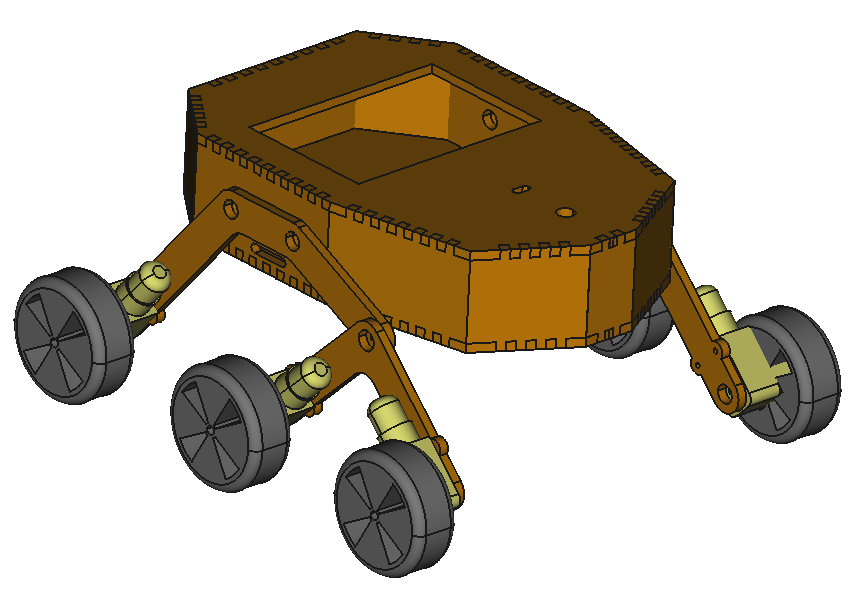
\includegraphics[width=.5\textwidth]{images/hw/wheele_stl}
	\caption{Modelo CAD del robot}
\end{figure}
\\
La disposición geométrica es la de un vehículo diferencial, con tres pares de ruedas, cada una con su respectiva pareja de motor y encoder.\\

\subsection{Motores DC}
 Los seis motores utilizados, a pesar de que deberían comportarse de forma parecida, presentan respuestas muy diferenciadas; para una señal de control idéntica cada uno de ellos muestran puntos de operación distintos y se observan respuestas ante escalón muy variadas. Sin embargo, 
 todos presentan un comportamiento común, una gran zona muerta que complicará mucho la operación del robot a velocidades extremadamente bajas. En concreto, con el convesor digital-analógico del microcontrolador seleccionado (más detalles en la seccion2.arduino), se pierde un 40\% de los bits del rango de salida a causa de este incoveniente.  
\subsubsection{Especificaciones}
\begin{itemize}
	\item Tensión de trabajo: 3-6 V.
	\item Corriente máxima: 120 mA.
	\item Dimesiones: 70x22x18 mm.
	\item Reductora: 48 revoluciones a una.
	\item Peso (sin ruedas): 29 gramos.
\end{itemize}

\newpage
A continuación, se mostrará la caracteristica estática obtenida para uno de los motores, la caracterización para el resto se ha realizado de forma análoga. 
\begin{figure}[h!]
	\centering
	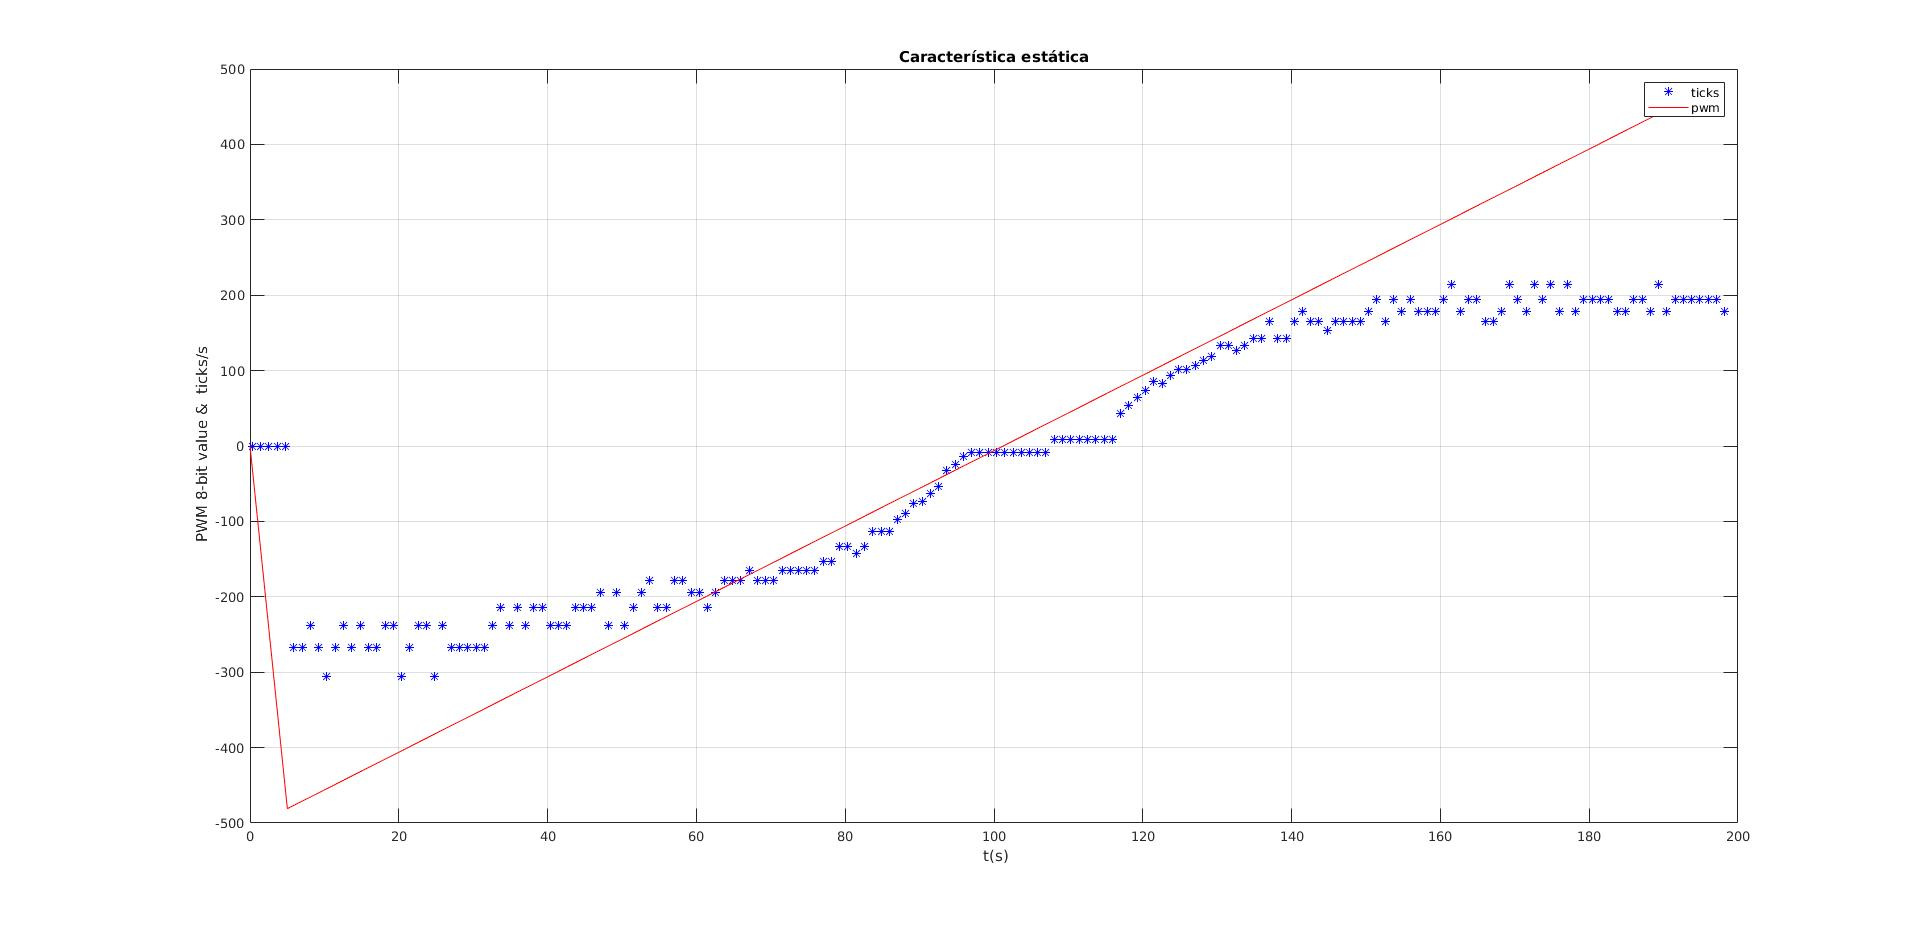
\includegraphics[width=.6\textwidth]{images/hw/estatica}
	\caption{Característica estática de un motor}
\end{figure}


\subsubsection{Drivers}
Se han empleado tres microchips L293D que integra cada uno dos puentes H. Estos puentes H nos permiten configurar la dirección de giro con dos señales digitales y la velocidad con otras dos señales analógicas.\\
Por comodidad y robustez, se ha diseñado en \textit{KiCad} una placa de circuito impreso muy simple que facilita el cableado y permite integrar algún 
componente pasivo (como diodos fly-back o capacidades de by-pass). \\
Gracias al laboratorio de electrónica este diseño ha sido revelado sobre una placa de una sola cara, obteniendo, como se aprecia en las imágenes, 
un acabado final bastante bueno.\\
 \begin{figure}[h!]
	 \centering
	 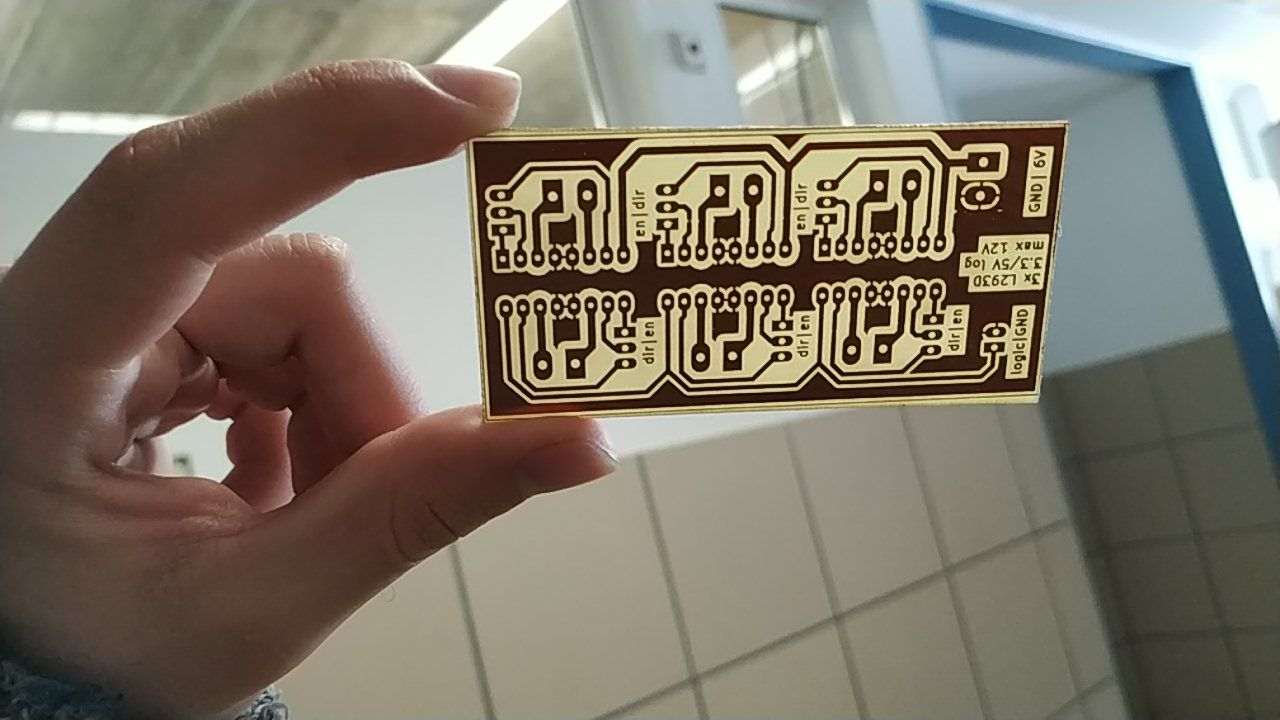
\includegraphics[width=.6\textwidth]{images/hw/pcb_img}
 	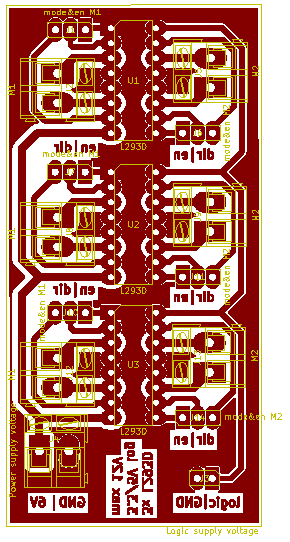
\includegraphics[width=.2\textwidth]{images/hw/pcb_kicad}
 	\caption{Diseño en KiCad de la PCB.}
 \end{figure}

 Los integrados requieren de una referencia de tensión lógica de 5V y una alimentación para los motores, que será a 6V. \\
Los 5V se sacarán del Arduino y los motores se alimentarán con una fuente externa de 6V y X A.

\newpage
\subsection{Encoders}\label{enc_hard}
Los sensores elegidos para medir la velocidad de cada rueda y estimar la posición y velocidad del robot, son unos sencillos encoders ópticos binarios junto a unos discos perforados. Al pasar la luz por una perforación del disco, 
que gira a la misma velocidad que la rueda, se manda una señal digital al micro. Contabilizando los flancos de subida o de bajada en cierto periódo de tiempo, y conociendo las dimensiones del disco, se obtiene una estimación de 
la velocidad.
 \begin{figure}[h!]
 	\centering
	 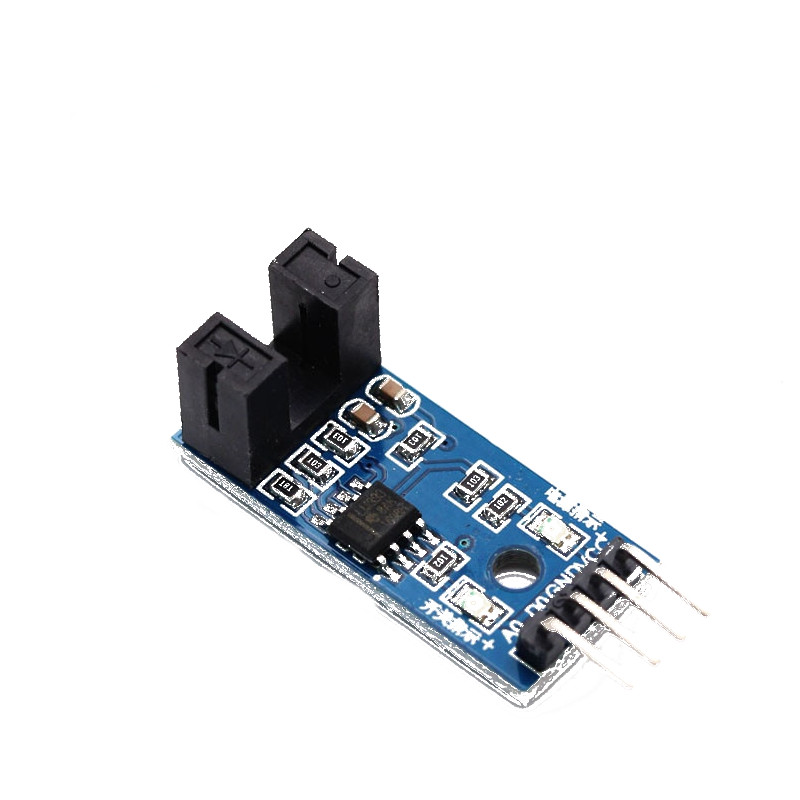
\includegraphics[width=.4\textwidth]{images/hw/encoder_img_rect}
	 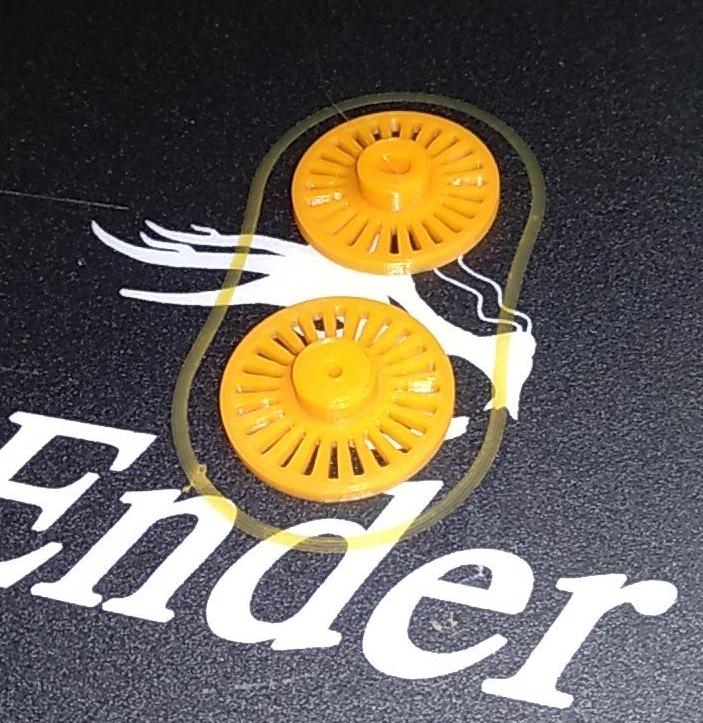
\includegraphics[width=.4\textwidth]{images/hw/encoder_stl}
 	\caption{Encoder óptico y disco empleados}
 \end{figure}

\subsection{IMU}\label{imu_hardw}
Como ya se ha mencionado con anterioridad, se ha escogido una IMU MPU-6050 de seis grados de libertad para obtener datos de las velocidades y aceleraciones del robot. El microchip contine varios subsitemas, de los cuales nos interesa resaltar especialmente:
\begin{itemize}
	\item Giroscópio (tres ejes), con un rango progamable de ±250, ±500, ±1000 y ±2000 °/s (grados / segundos).
	\item Acelerómetro (tres ejes), con un rango progamable de ±2g, ±4g, ±8g y ±16g.
	\item Conversores analógico-digitales de 16 bits para las salidas del giroscópio y del acelerómetro.
	\item Bus i2c para ejecutar operaciones de lectura y escritura en cualquier registro del chip a una frecuencia máxima de 400kHz.
	\item Bus de comunicación auxiliar que posibilita introducir un magnetómetro en el futuro sin modificar el conexianado de todo el sistema.
\end{itemize}
Puesto que la IMU consume muy poca potencia en todo momento, se puede alimentar sin problemas desde cualquier salida de referencia de la Raspberry. \\

\newpage
A continuación, se mostrará una imagen de la IMU conectada:
\begin{figure}[h!]
	\centering
	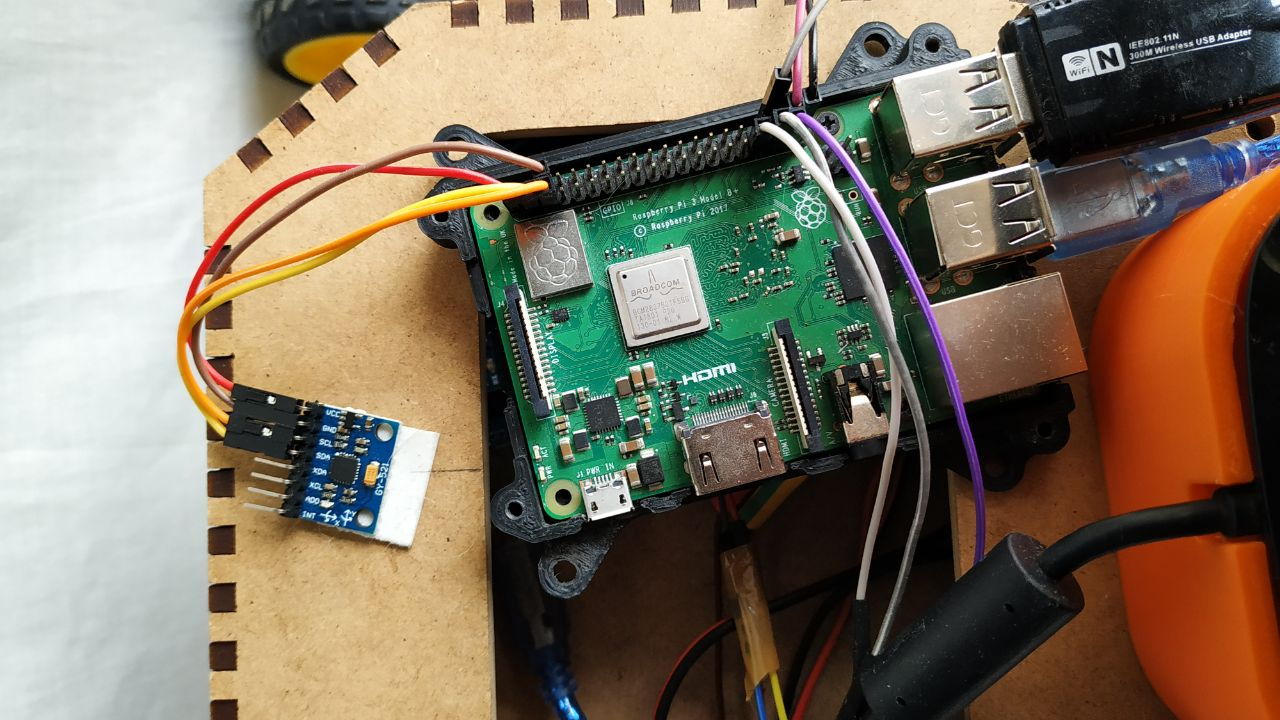
\includegraphics[width=.5\textwidth]{images/hw/rpi_imu}
	\caption{Conexionado entre la RPi y la IMU por $I^2C$}
\end{figure}

\subsection{Raspberry Pi}
Este \textit{single-board computer}, como se le denomina en inglés, alberga muchas posibilidades. En el centro de todas ellas se encuentra un procesado ARM Cortex-A53 de 64-bit a 1.4Ghz capaz de correr varias distribuciones de GNU/Linux. \\
Con la limitada potencia gráfica de la que dispone, y su único gigabyte de memoria RAM resulta necesario procesar los cálculos más complejos en otro sistema más potente.\\
El modelo utilizado (3B+) incluye WiFi 802.11n a 150Mbit/s máximo. Sin embargo, es conveniente usar una antena WiFi externa más potente para conseguir más rango de señal.\\
La Raspberry es alimentada a través de un puerto micro USB a 5V con una corriente máxima de 2.5A aunque su lógica funciona a 3.3V.

\subsection{Arduino Uno}
Por conveniencia se ha optado por una placa arduino, que además de un microcontrolador ATmega328p, integra un puerto usb con un chipset que facilita su programación y la comunicación serie con el mismo. Incluye también un cristal de cuarzo , que provee una fuente prescisa para la señal de reloj y resulta especialmente útil para implementar el control de bajo nivel.\\
El micro cuenta con una memoria flash progamable de 32 kilobytes y una eeprom de un kilobyte, que es más que suficiente para el uso que se le va a dar. Dos timers de 8 bits y otro de 16 bits generan las interrumpciones necesarias para controlar el tiempo real e implementar el control. De todas las 23 posibles entradas/salidas digitales del micro, se ocupan cuatro salidas para seleccionar el sentido de la marcha de los motores (dos para todos las ruedas de la izquierda y dos para las de la derecha) y seis canales PWM para controlar la velocidad individual de cada uno.\\
\begin{figure}[h!]
	\centering
	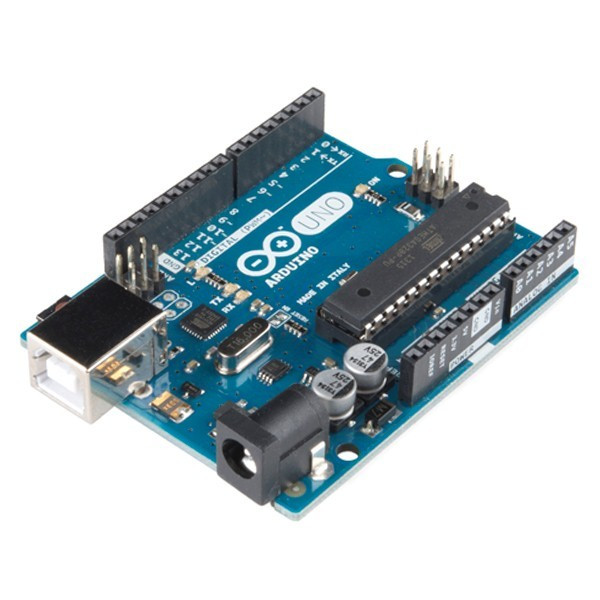
\includegraphics[width=.3\textwidth]{images/hw/arduino}
	\caption{Microcontrolador empleado para la comunicación a bajo nivel}
\end{figure}

La potencia eléctrica necesaria para que el micro, y sus periféricos, operen correctamente (5V y menos de 100mA) se obtienen por el puerto USB desde la Raspberry Pi, aprovechando el bus de comunicación serie.

\subsection{Cámara}
La \textit{Kinect for Xbox 360 V1} integra una cámara RGB y un sensor de profundidad de luz infrarroja estructurada. El rango del sensor de profundidad esta comprendido entre los 0.7 y los 6 metros.\\

\begin{figure}[h!]
	\centering
	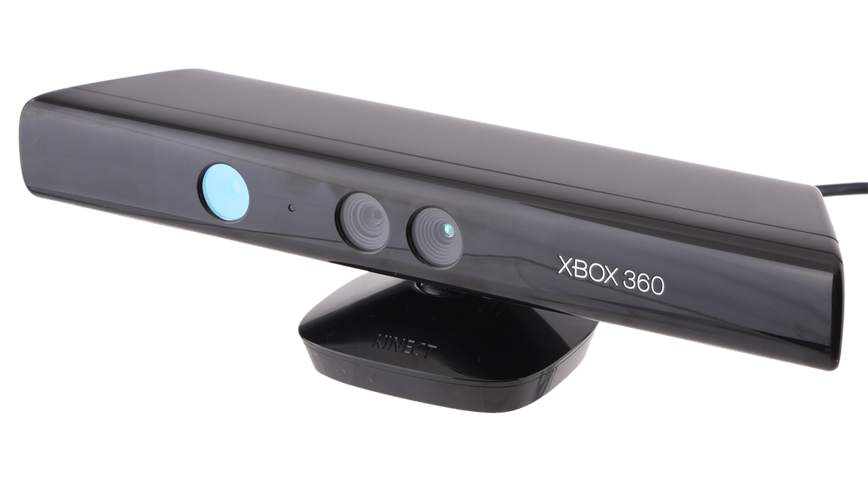
\includegraphics[width=.4\textwidth]{images/kinect}
	\caption{Cámara RGB-D Kinect}
\end{figure}

El campo de visión del dispositivo es de 57º horizontalmente y 43º en la vertical, aunque cuenta con un soporte motorizado que controla el \textit{pitch} de la camara. \\
La resolución máxima de la cámara es de 1280x1024 píxeles, pero la más usada es 640x480 píxeles puesto que el frame rate depende fuertemente de la resolución con la que se trabaje en los 30Hz.\\

El calculo de la profundidad lo realiza del siguiente modo a partir de la matriz proyectada:
\begin{figure}[h!]
	\centering
	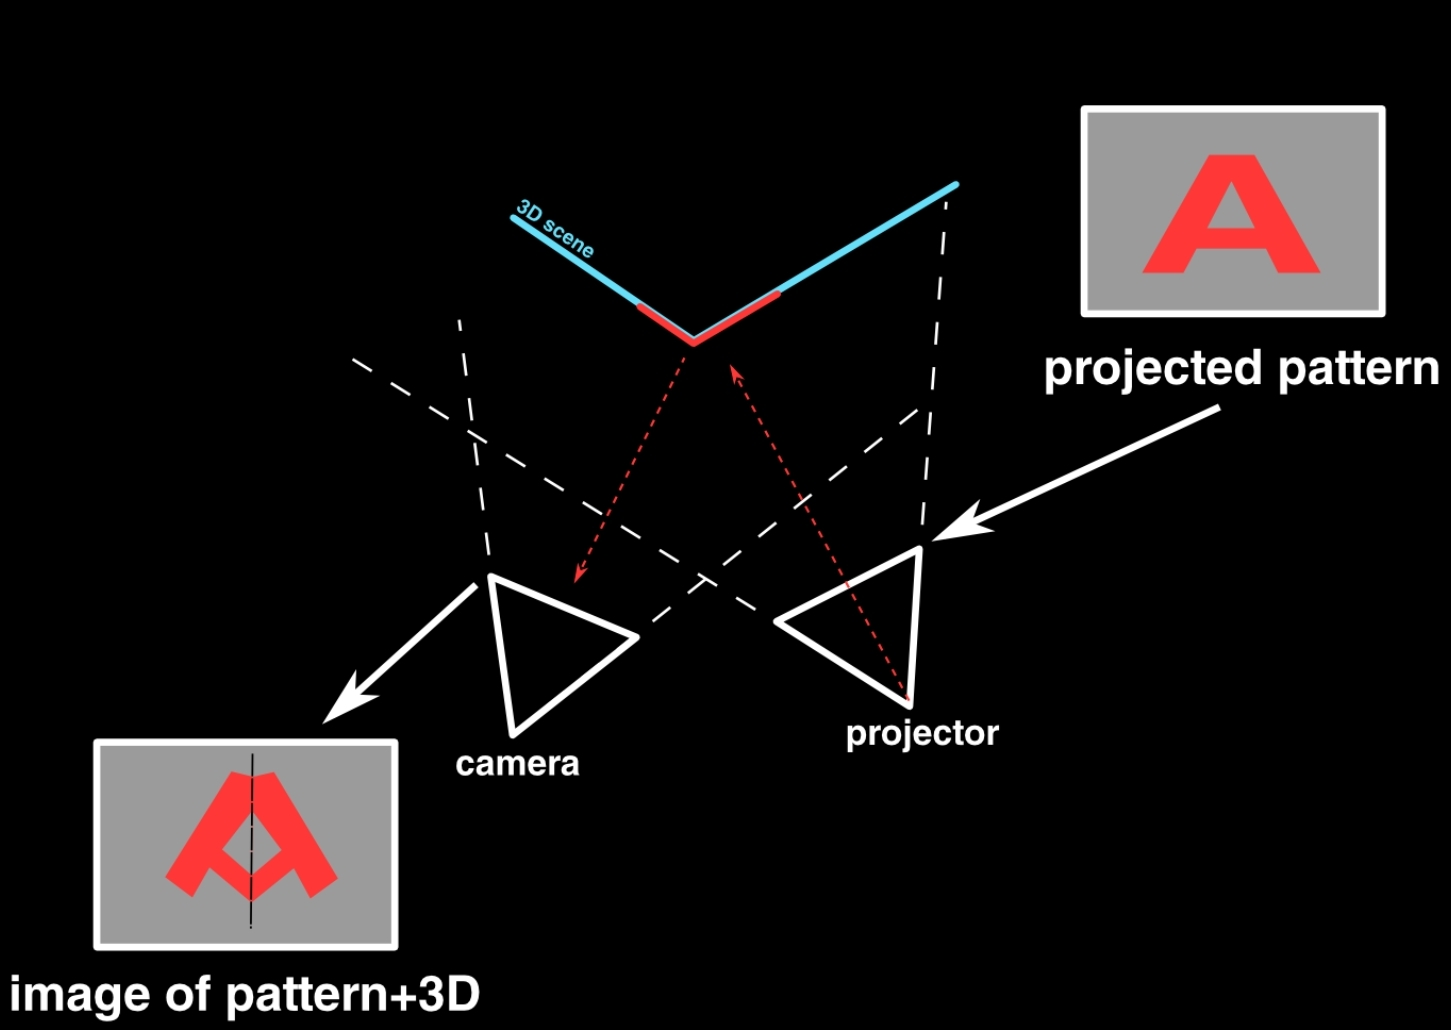
\includegraphics[width=.7\textwidth]{images/kinect_teo}
	\caption{Cámara RGB-D Kinect}
\end{figure}

\newpage
\subsection{Esquema de comunicación del hardware}
Debido a la multitud de entradas y salidas digitales y analógicas necesarias, al coste computacional de todo el sistema, y a la variedad de las comunicaciones, se plantea una configuración muy modular 
entre el ordenador de abordo (la \textit{Raspberry Pi}), los periféricos y la unidad de procesamiento para las partes más pesadas del software.\\
  \begin{figure}[h!]
  	\centering
  	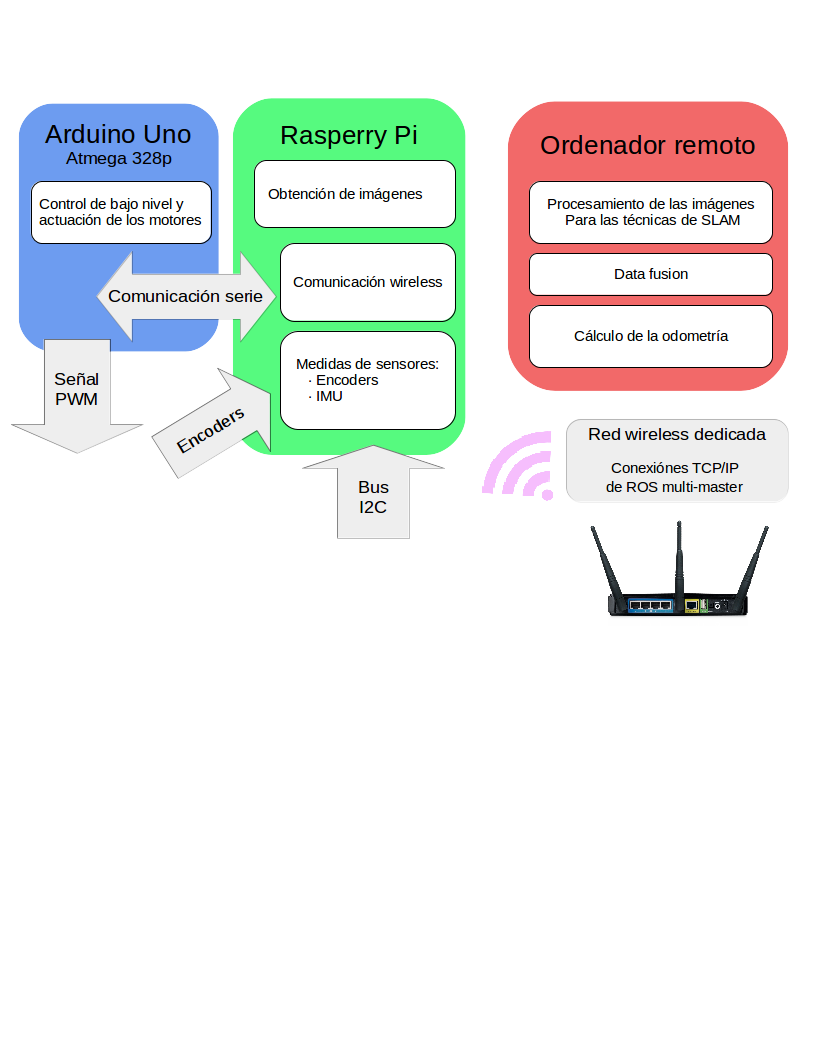
\includegraphics[width=.7\textwidth]{images/hw/wheele_esquema}
  	\caption{Esquema de conexionado de todos los componentes}
  \end{figure}